\chapter{\label{chap:scenarios}Cenários para Execução}

\begin{figure}[H]
\centering
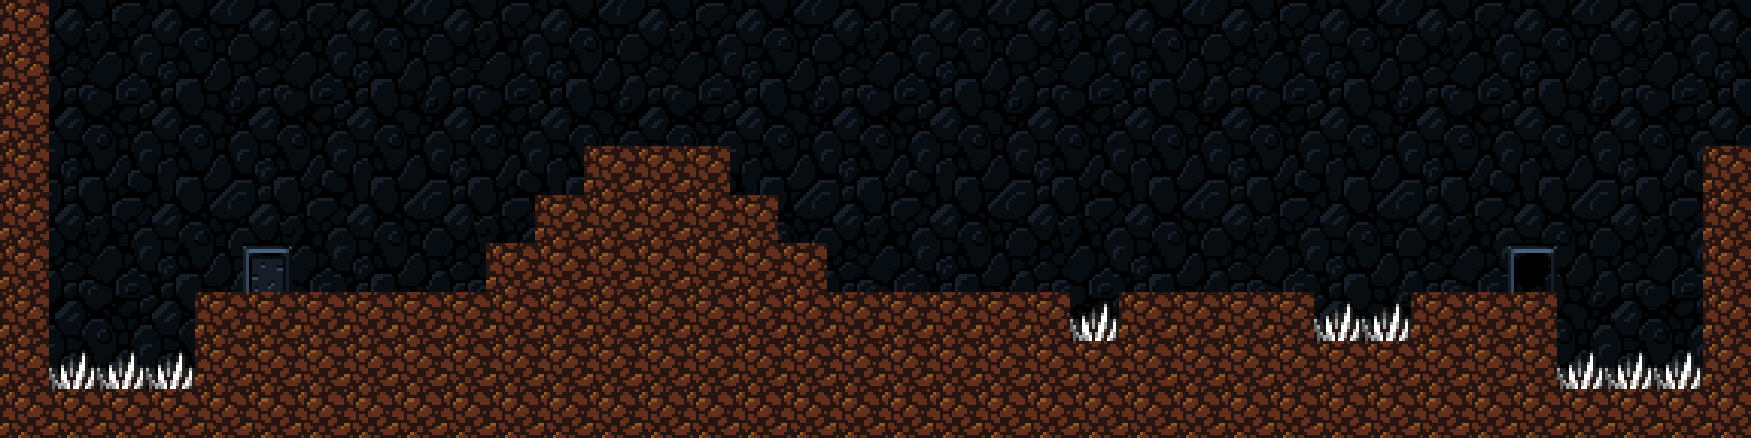
\includegraphics[width=\textwidth]{fig/levels/level1.pdf}
\caption{Level 1}
\label{fig:level1}
\end{figure}

\begin{figure}[H]
\centering
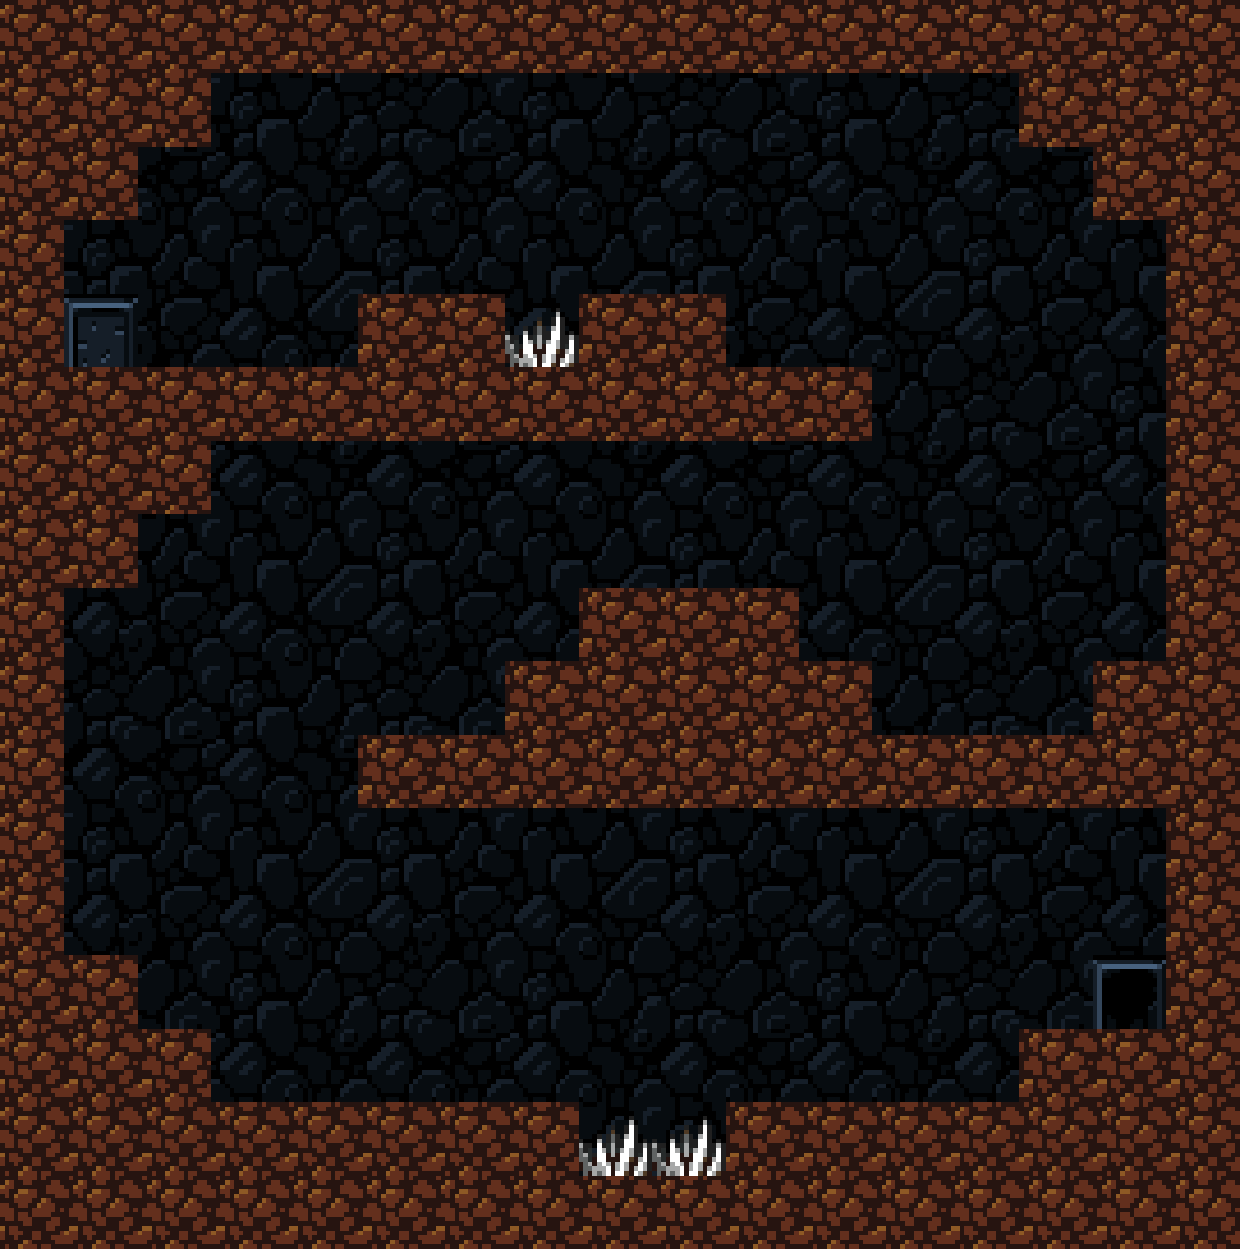
\includegraphics[width=\textwidth / 2]{fig/levels/level2.pdf}
\caption{Level 2}
\label{fig:level2}
\end{figure}

\begin{figure}[H]
\centering
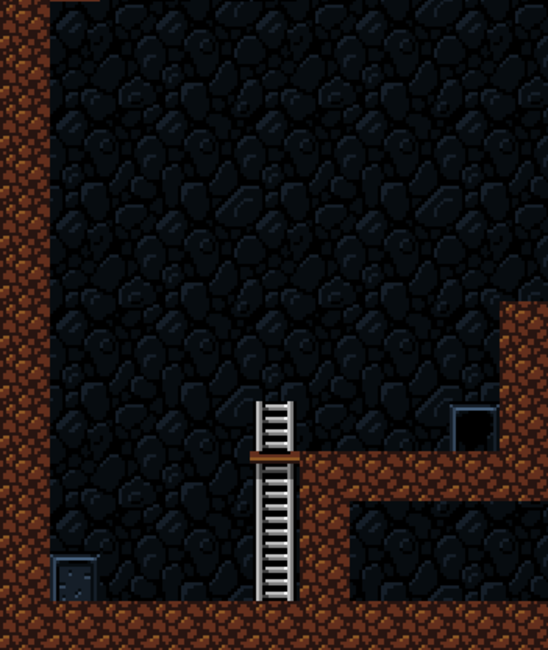
\includegraphics[width=\textwidth / 2]{fig/levels/extra1.pdf}
\caption{Extra 1}
\label{fig:extra1}
\end{figure}

\begin{figure}[H]
\centering
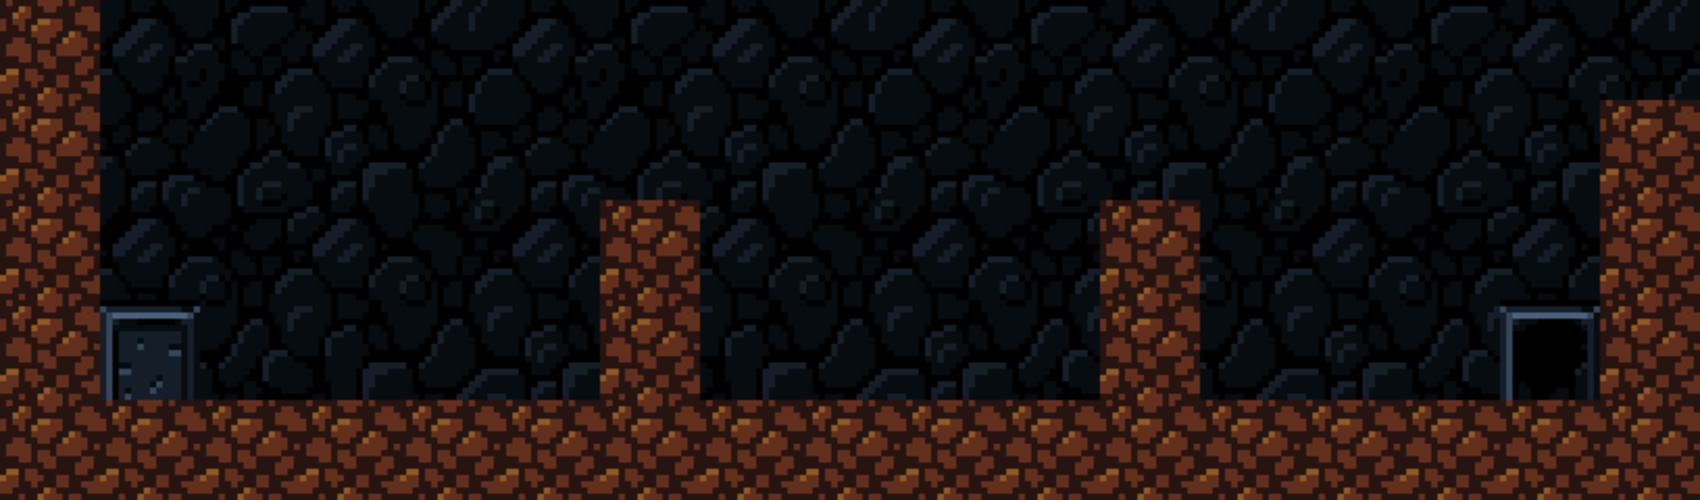
\includegraphics[width=\textwidth / 2]{fig/levels/extra2.pdf}
\caption{Extra 2}
\label{fig:extra2}
\end{figure}

\begin{figure}[H]
\centering
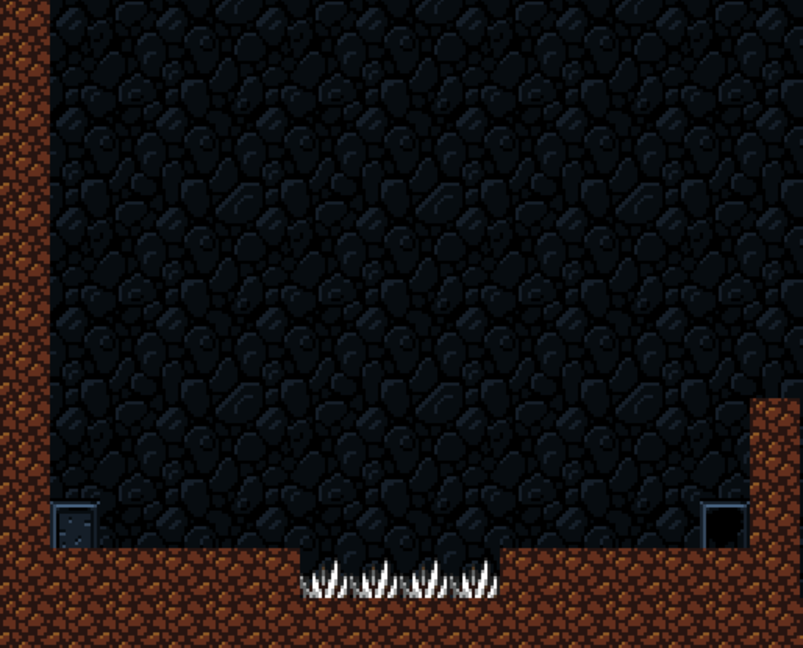
\includegraphics[width=\textwidth / 2]{fig/levels/extra3.pdf}
\caption{Extra 3}
\label{fig:extra3}
\end{figure}

\todoin[caption={Cenários para Execução}] {
\begin{itemize}
	\item Mapas escolhidos:
	\begin{itemize}
		\item Easy (apenas alguns obstáculos)
		\item Medium (obstáculos e deslocamento vertical)
		\item Hard (mapa normal, gerado)
		\item Detalhar parâmetros de execução e critério de parada de cada mapa
	\end{itemize}

	\item Mapas adicionais (para teste de features):
	\begin{itemize}
		\item Motivação (tempo curto para explorar itens adicionais)
		\item Explorar corrida do bot
		\item Agarrando na parede
		\item Escadas
		\item Matar inimigos
		\item Coletar tesouros
		\item Detalhar parâmetros de execução e critério de parada de cada mapa
	\end{itemize}
\end{itemize}
}
